\documentclass{standalone}
\usepackage{tikz}
\usepackage{pgfplots}

\begin{document}
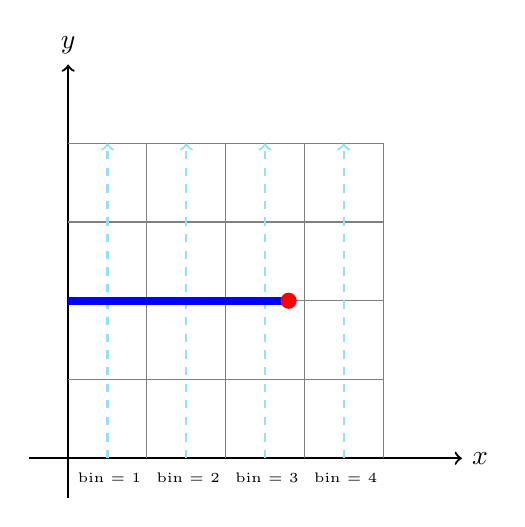
\begin{tikzpicture}[scale=1]

    % Draw axes with slightly extended lines to match sdistance
    \draw[thick,->] (-0.5,0) -- (5,0) node[right] {$x$}; % Extended x-axis left of origin
    \draw[thick,->] (0,-0.5) -- (0,5) node[above] {$y$}; % Extended y-axis below origin
    
    % Draw grid (4x4 box)
    \foreach \x in {1,2,3,4} {
        \draw[gray, thin] (\x,0) -- (\x,4);
    }
    \foreach \y in {1,2,3,4} {
        \draw[gray, thin] (0,\y) -- (4,\y);
    }
    
    % Add x-labels
    \node[font=\tiny] at (0.525,-0.25) {bin = 1};
    \node[font=\tiny] at (1.525,-0.25) {bin = 2};
    \node[font=\tiny] at (2.525,-0.25) {bin = 3};
    \node[font=\tiny] at (3.525,-0.25) {bin = 4};
    
    % Draw customizable vertical arrows (adjust the coordinates as needed)
    \draw[cyan!40, thick,->, dashed] (0.5,0) -- (0.5,4); % Arrow in column 1
    \draw[cyan!40, thick,->, dashed] (1.5,0) -- (1.5,4); % Arrow in column 2
    \draw[cyan!40, thick,->, dashed] (2.5,0) -- (2.5,4); % Arrow in column 3
    \draw[cyan!40, thick,->, dashed] (3.5,0) -- (3.5,4); % Arrow in column 4
    
    % Draw the blue cylinder-like curve (middle of the grid, adjustable)
    \draw[blue, line width=1mm] (0,2) -- (2.8,2);  % Blue line replacing the red one
    \draw[blue, line width=1mm] (3,2) -- (3,2);    % Connecting the third and fourth columns here
    
    % Add a red circle slightly thicker than the blue line
    \filldraw[red, thick] (2.8,2) circle (2.5pt);  % Circle at the end of the blue line (you can adjust size)
    
    \end{tikzpicture}
    \end{document}